\section{Opgave 2}

\subsection{Specifikation}
Der ønskes et program der kan vise et udsnit af mandelbrotmængden i et vindue. Mængden skal kunne farvelægges med 
tilfældige farver eller med farver angivet i en fil. Brugeren skal kunne bevæge sig rundt i mængden med musen og 
indtaste kommandoer i konsollen der tillader brugeren at ændre på figurstørrelsen, udsnittet af mængden brugeren 
ser osv.. \\

Der er givet en fuldstændig specifikation af klassen Complex, der fungerer som en container for komplekse tal, 
og enkelte regneoperationer der kan udføres på dem. \\

NB: Da det ikke er specificeret hvilken version af java runtime miljøet der skal understøttes, anvendes i mandelbrot programmet funktioner der kun understøttes i JRE version 1.7 og frem.
\subsection{Design}
I henhold til specifikation opstilles følgene klasser
\begin{itemize}
    \item Mandelbrot; main-klasse til håndtering af grafik og interaktion med brugeren.
    \item ColorGenerator; klasse til håndtering af farver.
    \item Complex; Container til komplekse tal og enkelte regneoperationer.
\end{itemize}

\subsubsection{Complex klassen}
Complex klassen indeholder to felter af typen double, disse repræsenterer den imaginære og reelle del af et komplekst tal.
Da klassen er en utility klasse ses dens metoder nedenfor så kildekolden til Mandelbrot kan læses uden at kende til kildekoden i complex.
\begin{itemize}
    \item public Complex(); Konstruktør til at oprette et komplekst tal med værdien 0 + 0i.
    \item public Complex( double re, double im ); overloadet konstruktør til at oprette et komplekst tal med værdien re +im i
    \item public Complex( Complex z ); overloadet konstruktør til at oprette et komplekst tal identisk med z.
    \item public double getRe()/getIm(); getter metoder til re og im felterne.
    \item public double abs(); returnerer absolutværdien som en double.
    \item public Complex plus( Complex other ) returnerer værdien af addition mellem other og objektet metoden kaldes på.
    \item public Complex times( Complex other ) returnerer værdien af multiplikation mellem other og objektet metoden kaldes på
\end{itemize}
Klassen bruges som utility klasse i Mandelbrot programmet.

\subsubsection{ColorGenerator klassen}
Klassen ColorGenerator indeholder metoder til at håndtere farver af typen java.awt.Color. Klassen kan generere et
sæt af random farver, eller indlæse et sæt af farver fra en fil. Dette er nødvendigt eftersom specifikationen kræver
at mandebrotprogrammet kan tegne mandelbrotmængden med tilfældige farver, eller farver indlæst fra en fil. \\


Da klassen er en utility klasse ses dens metoder nedenfor så kildekoden til Mandelbrot kan læses uden at kende til kildekoden i ColorGenerator.
\begin{itemize}
    \item public Color[] generateRandomColorMap( int numColors ) Returnerer en kopi af et array med tilfældige unikke farver af størrelse numColors. Smider IllegalArgumentException hvis numColors er \textless = 0 eller så stor at køretiden er uendelig. 
    \item public Color generateRandomColor() Returnerer en tilfældig farve.
    \item public Color[] generateColorMapFromFile( String fileName ) Returnerer en kopi af et array med farver specificeret i en fil. Smider IOException hvis der sker en fil i fillæsningen.
\end{itemize}

ColorGenerator klassen anvedes i Mandelbrot programmet til at håndtere hvilken farve et specifikt punkt skal tegnes med.

\subsubsection{Mandelbrot klassen}
Mandelbrot klassen er den statiske klasse der indeholder mandelbrot-programmets kontrolflow. Ydermere indeholder Mandelbrot klassen metoder til at håndtere input fra brugeren og rendering af mandelbrotsættet. \\

Programflowet er som følger:
\begin{enumerate}
    \item Initialiser programvindue med standardværdier.
    \item Tegn den del af mandelbrotsættet der er i fokus.
    \item Tjek om brugeren har indtastet konsolinput, hvis ja; opdater det viste udsnit af mandelbrotmængden.
    \item Tjek om brugeren trykker på musen, hvis ja; opdater det viste udsnit af mandelbrotmængden.
    \item Gå til 2.
\end{enumerate}

Når programmet køres åbnes således et vindue med de arbitrære standard værdier hvorefter brugeren kan navigere rundt i mandelbrot sættet med musen, eller med konsol kommandoer. \\
Der er følgene konsolkommandoer til rådighed.
\begin{itemize}
    \item set figuresize *int x* ændrer figurstørrelsen i vinduet til x*x.
    \item set gridsize *int x* ændrer antallet af punkter i det komplekse plan der evalueres til x*x.
    \item set sidelength *double x* ændrer sidelængden af viste udsnit af det komplekse plan til x.
    \item set center *double x* *double y* ændrer centrum af den viste punktmængde til x + iy.
    \item set zoomfactor *double x* ændrer zoomfactoren der bruges ved museklik til x. x<1 zoomer ud.
    \item set colormap *string map* ændrer farvekoden til farver specificeret i filen med stien map. Hvis der indtastes ''random'' skiftes der til en tilfældigt genereret farvekode.
\end{itemize}
Hvis programmet ikke genkender en kommando printes ''No such command'' til konsollen og kommandoen ignoreres. Ligeledes printes ''Error parsing command'', plus den sidst genkendte del af en kommando,  hvis programmet ikke kan genkende de indre dele af en kommando.\\

Ovenstående er ikke en optimal måde at håndtere museinput på, da der kun udføres et tjek hver gang programmet kører igennem sit update-loop. Dette medfører at museklik der eksekveres imens programmet renderer et nyt billede, eller håndterer konsolinput ikke bliver registreret. En bedre løsning ville være at have en tråd dedikeret til bruger input.
Denne tråd ville stille alle indtastede kommandoer op på en stack der så kunne tømmes når mainprogrammet har tid.\\
Konsolinput håndtering lider ikke af samme problem da der kan laves en buffer som fyldes op imens programmet eksekverer anden kode.

\subsection{Testing}

Til test af Complex klassen er der skrevet en klasse TestComplex der anvender assert statements til at verificere at alle metoderne virker korrekt. \\
ColorGenerator er sværere at teste med assert statements, men det er verificeret at de to metoder der kaster exceptions, kaster dem på de korrekte betingelser. \\
Korrektheden af resten af ColorGenerator verificeres i testen af mandelbrot programmet. \\


Main programmet er et interaktivt program og vil derfor blive testet ved at forsøge at lave en inputsekvens der dækker hele programmet. Nedenfor ses en enkelt input sekvens og snapshots af det renderede billede for hver ændring.
\lstinputlisting[caption={Inputsekvens til madelbrot programmet}, label=mandelseq]{mandel.log}
Disse input afprøver hele programmets featureset. En listing med fejlinput ses nedenfor.

\begin{lstlisting}[caption=fejlinput i mandelbrot konsol]
java Mandelbrot
foo
No such command
set foobar
Error parsing command set
set colormap foo
Error loading colormap
set gridsize 9999999999999999999999999999999999999999
Error parsing command set gridsize
set gridsize 42.0
Error parsing command set gridsize
\end{lstlisting}
Det ses her at programmet håndterer fejlinput korrekt. Både ikke genkendelige kommandoer og typefejl.
\begin{figure}
    \centering
    \begin{subfigure}[b]{0.3\textwidth}
        \centering
        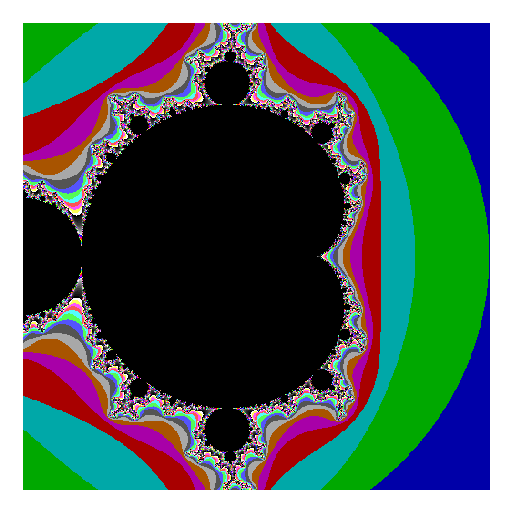
\includegraphics[width=\textwidth]{pictures/M0.png}
        \caption{ Render af default værdier }
    \end{subfigure}
    \begin{subfigure}[b]{0.3\textwidth}
        \centering
        
\includegraphics[width=\textwidth]{pictures/M2.png}
        \caption{ Snapshot efter linje 2 i listing \ref{mandelseq} }
    \end{subfigure}
    \begin{subfigure}[b]{0.3\textwidth}
        \centering
        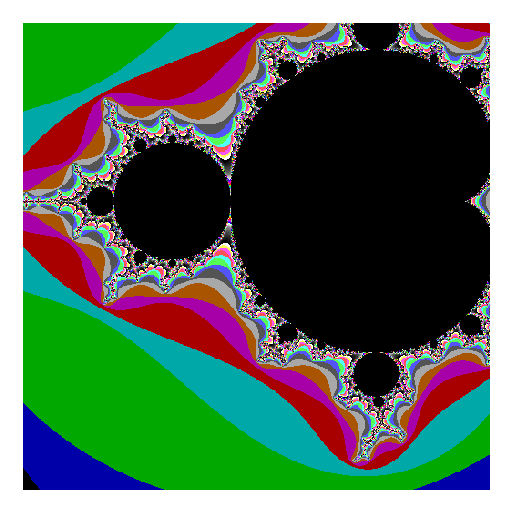
\includegraphics[width=\textwidth]{pictures/M3.png}
        \caption{ Snapshot efter linje 8 i listing \ref{mandelseq}, eksempel på museinput. }
    \end{subfigure}

    \begin{subfigure}[b]{0.3\textwidth}
        \centering
        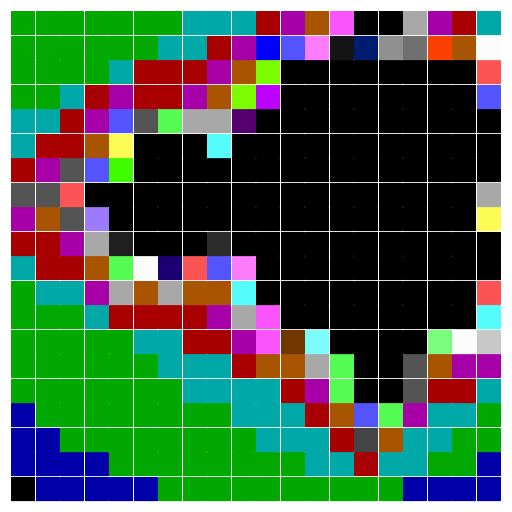
\includegraphics[width=\textwidth]{pictures/M4.png}
        \caption{ Snapshot efter linje 9 i listing \ref{mandelseq}. }
    \end{subfigure}
    \begin{subfigure}[b]{0.3\textwidth}
        \centering
        
\includegraphics[width=\textwidth]{pictures/M5.png}
        \caption{ Snapshot efter linje 11 i listing \ref{mandelseq}. }
    \end{subfigure}
    \begin{subfigure}[b]{0.3\textwidth}
        \centering
        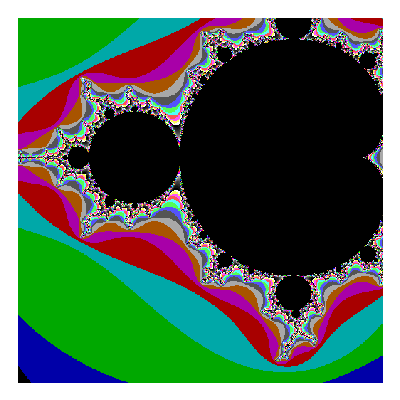
\includegraphics[width=\textwidth]{pictures/M6.png}
        \caption{ Snapshot efter linje 13 i listing \ref{mandelseq}}
    \end{subfigure}

    \begin{subfigure}[b]{0.3\textwidth}
        \centering
        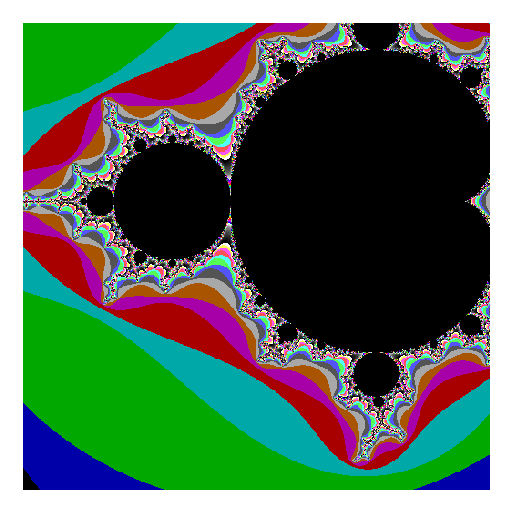
\includegraphics[width=\textwidth]{pictures/M7.png}
        \caption{ Snapshot efter linje 15 i listing \ref{mandelseq}.}
    \end{subfigure}
    \begin{subfigure}[b]{0.3\textwidth}
        \centering
        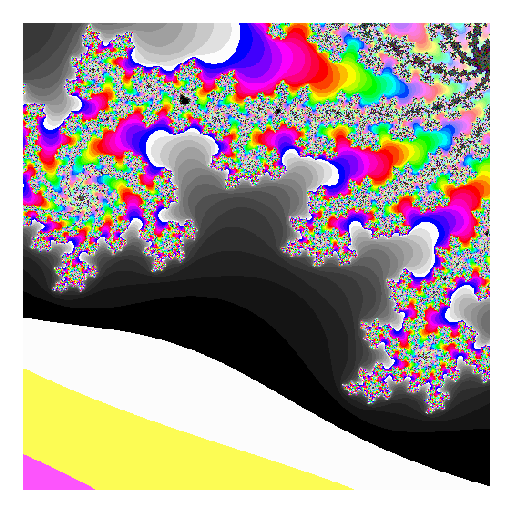
\includegraphics[width=\textwidth]{pictures/M8.png}
        \caption{ Snapshot efter linje 19 i listing \ref{mandelseq}.}
    \end{subfigure}
    \begin{subfigure}[b]{0.3\textwidth}
        \centering
        
\includegraphics[width=\textwidth]{pictures/M9.png}
        \caption{ Snapshot efter linje 21 i listing \ref{mandelseq}.}
    \end{subfigure}

    \begin{subfigure}[b]{0.3\textwidth}
        \centering
        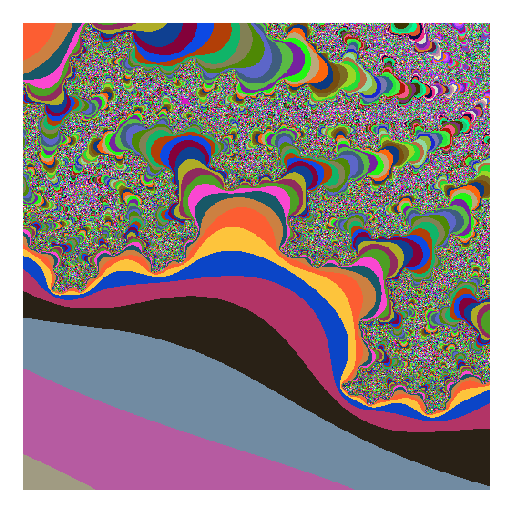
\includegraphics[width=\textwidth]{pictures/M10.png}
        \caption{ Snapshot efter linje 23 i listing \ref{mandelseq}.}
    \end{subfigure}
\end{figure}
